%#######################################################################
%
% Introduction and motivation for open tool support and VDM + UML
%
\section{Introduction}
%-----------------------------------------------------------------------
%
% Motivation
%
\frame
{
  \frametitle{Motivation}

%\begin{block}<+->{Abstract}
%A short introduction to the Overture project showing how to bootstrap the tools for VDM. Short demo of the Editor and Debug execution.
%\end{block}
\begin{center}
  \begin{itemize}
	%\itemsep=1cm
  		\item Limited tool support
  		\item Best of both by combining VDM and UML
  		\item Provide an easy to use and extensible user interface
  \end{itemize}
\end{center}
}



%
% Goal
%
\frame
{
  \frametitle{Goal}

\begin{center}
  \begin{itemize}
	%\itemsep=1cm
  		\item Provide a connection between VDM and UML
  		\item Display a VDM static structure diagram (Class Diagram)
  		\item Creation of Combinatorial Test statements from a dynamic diagram (Sequence Diagram)
  		\item Integrate the transformation tool into Eclipse
  		\item Open source
	  	
  \end{itemize}
\end{center}
}

%-----------------------------------------------------------------------
\subsection{Open Source Tool support}
%-----------------------------------------------------------------------
%
% Improce Tools support
%
\frame
{
  \frametitle{Improve tool support}
\begin{center}
  \begin{itemize}
	%\itemsep=1cm
  		\item Improve tools support for VDM development
  		\item Only one commercial tool for VDM (VDM Tools by CSK)
  		\item UML transformation in VDM Tools - Rose VDM Link first release (1997)
  		\item Enable UML tool support for VDM.
	  	
  \end{itemize}

\end{center}
}

%-----------------------------------------------------------------------
\subsection{Vienna Development Method}
%-----------------------------------------------------------------------
%
% VDM
%
\frame
{
  \frametitle{The Vienna Development Method}

\begin{center}
	\begin{block}<+->{Not created yet}
	Some thing about VDM
	\end{block}
  \begin{itemize}
	%\itemsep=1cm
  		\item VDM Specification Language (VDM-SL) ISO released in '96
  		\item Extended in 1992-94 with object oriented structure and concurrency handling (VDM++).
  		\item Last extension made for distributed real-time systems (VICE).
  		\item Two most significant tool suites. (VDM Tools and Overture)
	  	
  \end{itemize}

\end{center}
}

%
% Small VDM example
%
\frame
{
  \frametitle{Some VDM example}

\begin{center}

\vdmSpecLineNum{ClassDiagramOverview.vpp}{VDM classes with collections.}{VDM:Collections}

\end{center}
}

%-----------------------------------------------------------------------
\subsection{Unified Modeling Language}
%-----------------------------------------------------------------------
%
% UML
%
\frame
{
  \frametitle{Unified Modeling Language - UML}

\begin{center}

	\begin{block}<+->{Not created yet}
	Some thing about UML
	\end{block}

\end{center}
}


%
% Small VDM example
%
\frame
{
  \frametitle{Some UML example}

\begin{center}

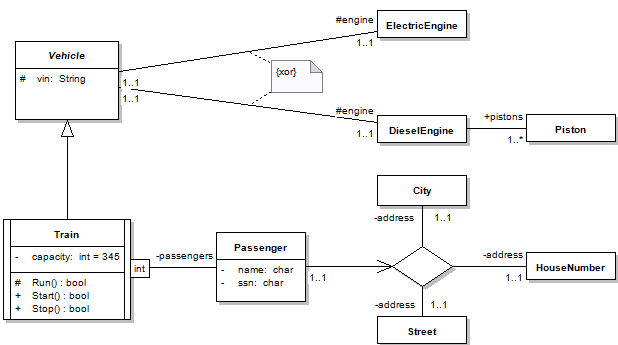
\includegraphics[width=\textwidth]{images/ClassDiagramOverview.png}

\end{center}
}
